\documentclass[tikz,border=10pt]{standalone}
\begin{document}
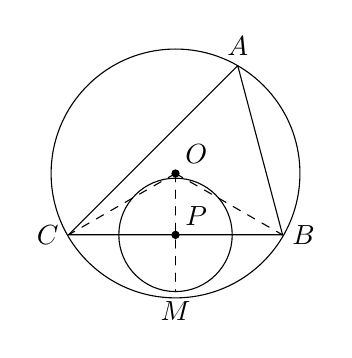
\begin{tikzpicture}[scale=1, line cap=round, line join=round]
\coordinate (O) at (2.03,-2.00);
\coordinate (A) at (2.82,-0.63);
\coordinate (C) at (0.67,-2.78);
\coordinate (B) at (3.39,-2.78);
\coordinate (P) at (2.03,-2.78);
\coordinate (M) at (2.03,-3.50);

\draw (O) circle (1.58);
\draw (A) -- (B) -- (C) -- cycle;
\draw (C) -- (B);
\draw[dashed] (O) -- (C);
\draw[dashed] (O) -- (B);
\draw[dashed] (O) -- (M);
\draw (P) circle (0.72);

\fill (O) circle (1.5pt);
\fill (P) circle (1.5pt);

\node[above] at (A) {$A$};
\node[above right] at (O) {$O$};
\node[above right] at (P) {$P$};
\node[below] at (M) {$M$};
\node[left] at (C) {$C$};
\node[right] at (B) {$B$};
\end{tikzpicture}
\end{document}
